\begin{figure}[h]
	\begin{center}
		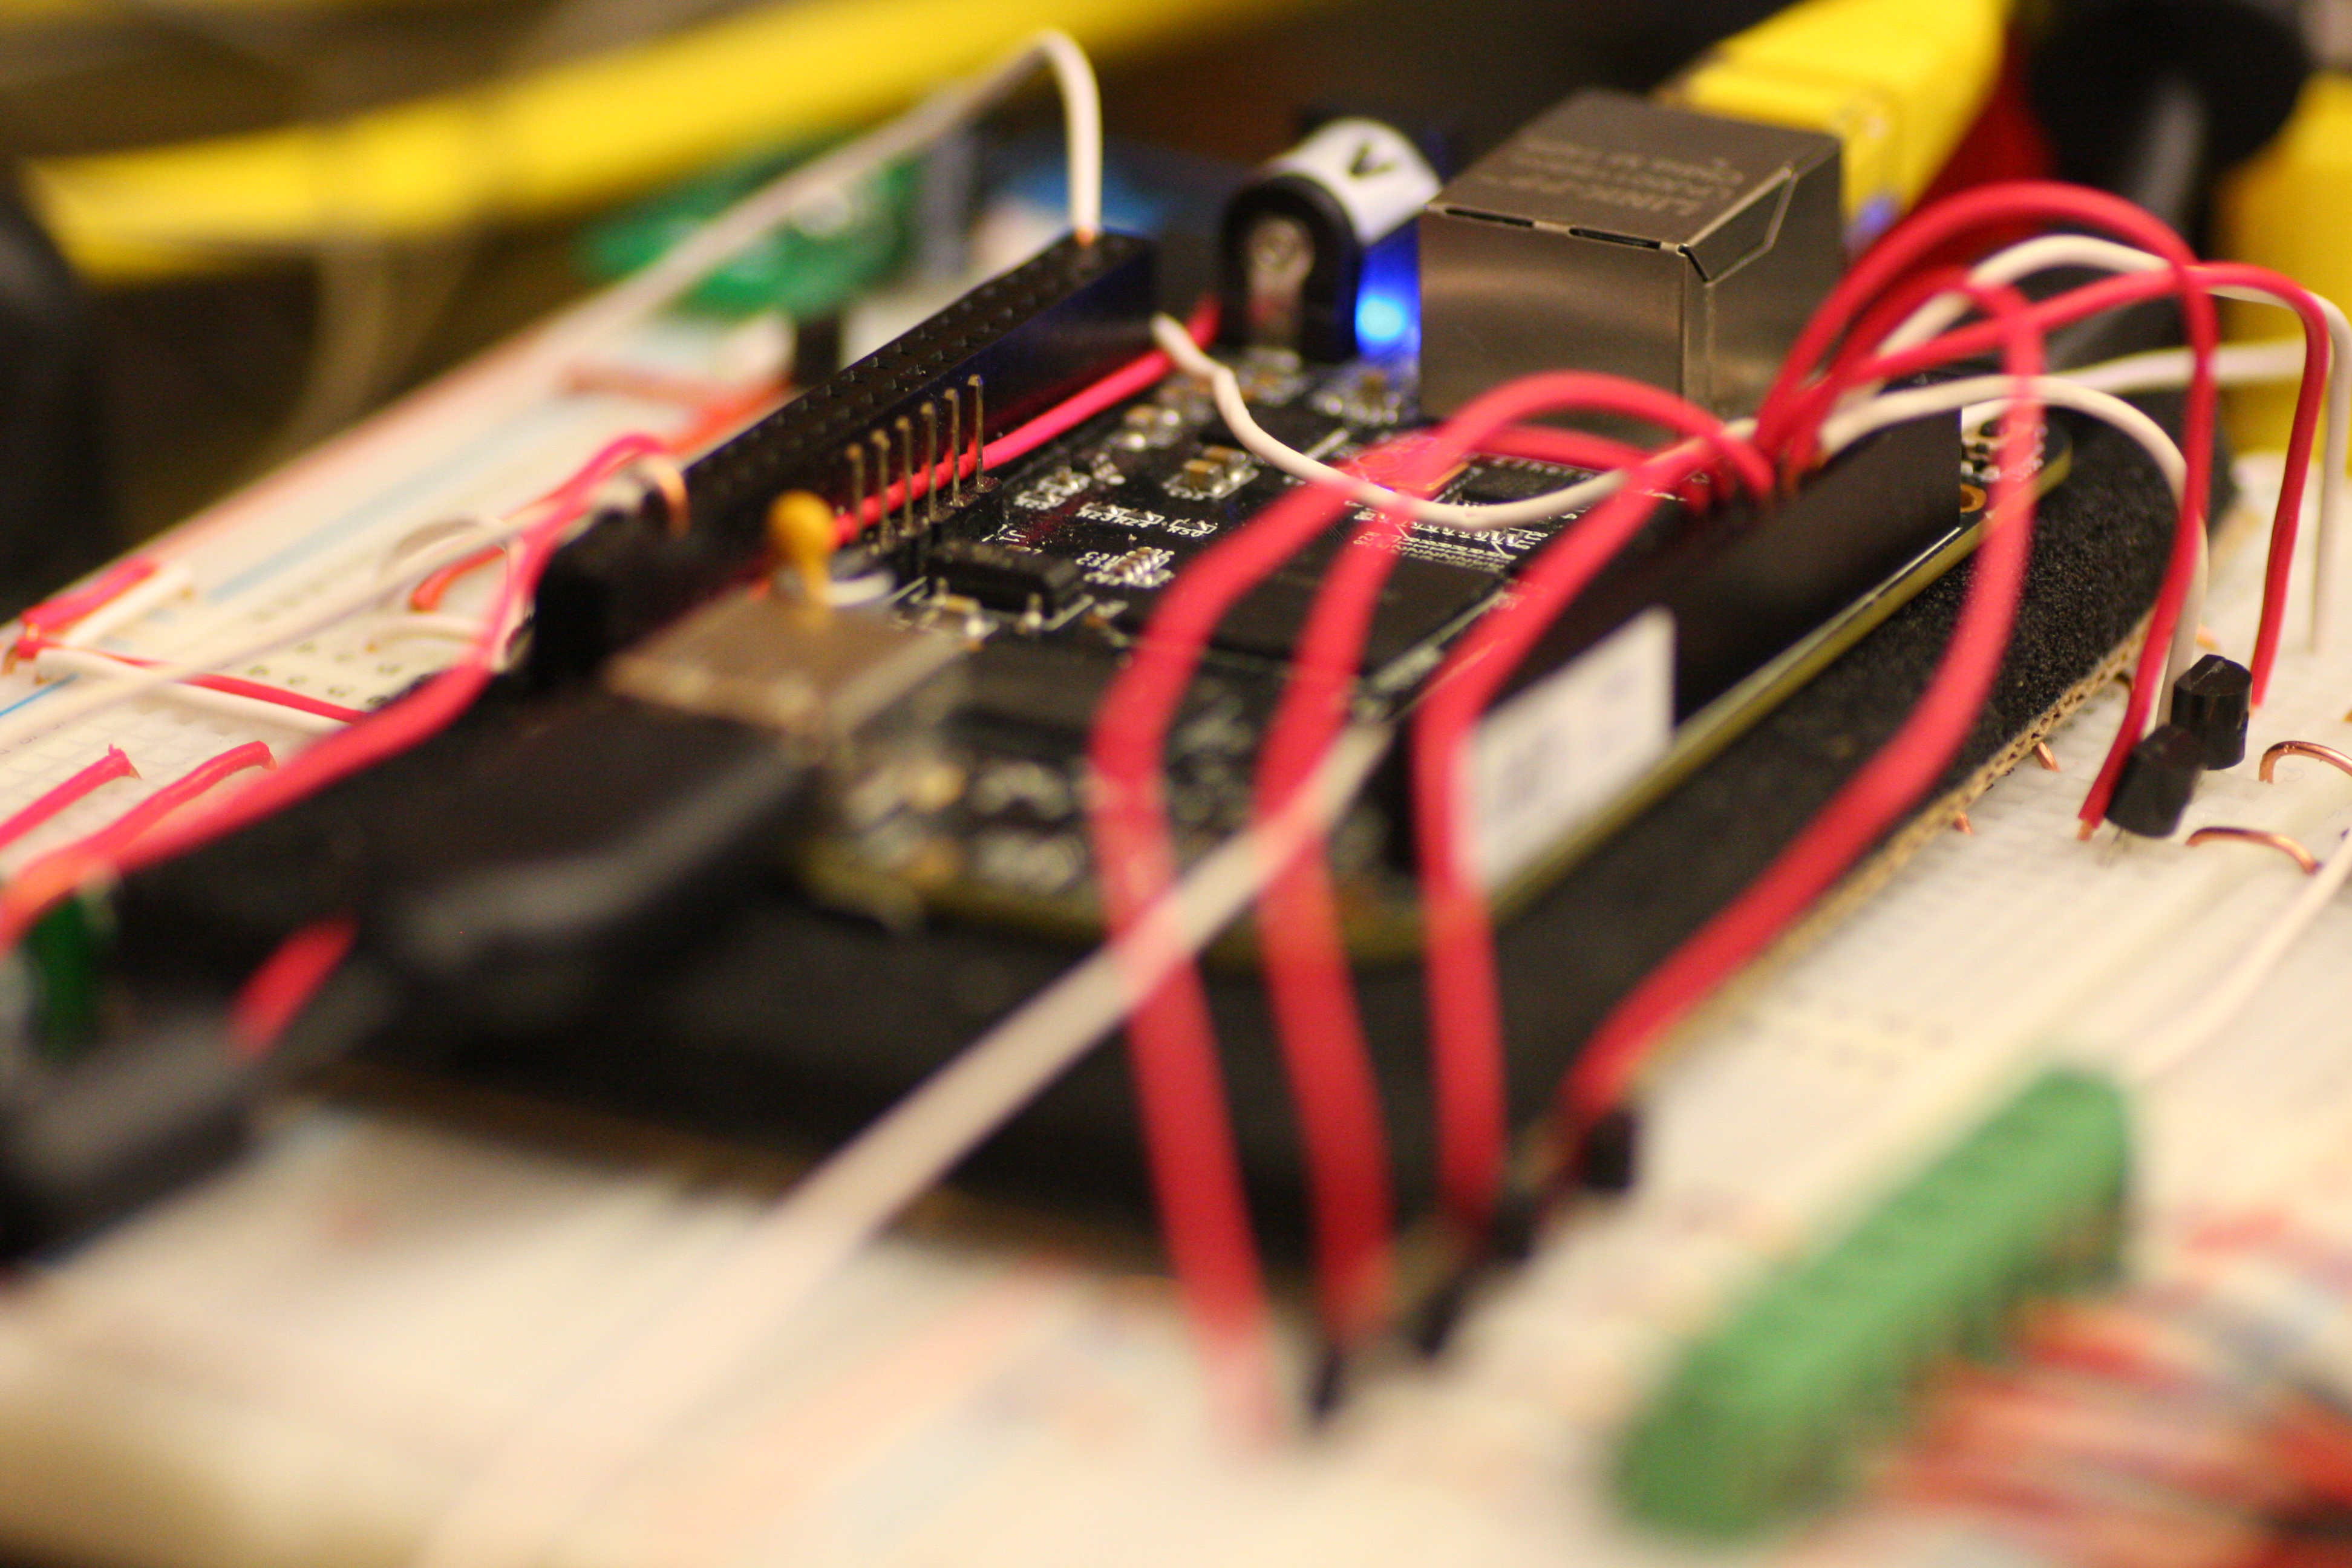
\includegraphics[width=\textwidth]{breadboard}
		\caption{Circuit mounted on breadboard side view}
		\label{Fig:circuitsfumatp}
	\end{center}
\end{figure}
For what concern the sensors acquiring paths, unfortunately, rigorous experiments have not been done. This is due to the end of my six months period. What I can say for those parts is that from the experiment that I made (not in a microfluidic or biomedical context) the results appear acceptable.

	While, in order to try the reverse control from the Google Glass to the electrovalves we made different kind of experiments.
	
	\section{LED Experiments}
	 First of all we tried the circuit on a breadboard using LEDs instead of electrovalves. The aim of this step is to demonstrate that the firmware running on the Beaglebone Black, the Java code running on the Google Glass and the Python code running on the Google App Engine (used to store the information about the electrovalves status) work well.\\
	Moreover the LED and the electrovalve have basically the same behavior so, if everything works well with the LEDs, there are all the reasons to believe that everything is going to work well with the electrovalves, too.\\
	
	The circuit that actually drives the LEDs is very simple, and it is based on a MOS transistor (\href{http://www.onsemi.com/pub_link/Collateral/BS170-D.PDF}{\textit{BS170}}) used as a switch voltage-controlled, as shown in (Fig.\ref{Fig:driverLED}).
	
	\begin{figure}[h]
		\centering
		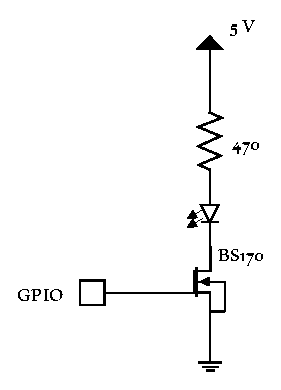
\includegraphics[]{Driver/driverLED}
		\caption{Driver for LED}
		\label{Fig:driverLED}
	\end{figure}
	
	The (Fig.\ref{Fig:circuitLED}) shows the circuit used for this step of testing. As can be seen the number of LEDs used is eight, the same number of electrovalves that can be driven from this system.\\
	In order to test all of them we made 2 different kind of trials:
	\begin{enumerate}
		\item \textit{In order turning on\&off}, first all the LEDs are turned on starting from the first one (on the top right corner) to the last one (on the bottom left corner). Then the LEDs are turned off following the same order.\\The result of this can bee watched in  \href{http://youtu.be/iYeAMpxM9uI}{\textbf{this}} video.
		\item \textit{Out of order turning on\&off}, in this trial, like before, all the LEDs start from a condition where all of them are off and then we turned on and off all the LEDs, but in this case following a random order.\\ The result of this can bee watched in  \href{http://youtu.be/mIoylW334Ck}{\textbf{this}} video.
	\end{enumerate}
	
	
	\begin{figure}[h]
		\centering
		\includegraphics[scale=.21]{Experiments/ledBoard}
		\caption{LEDs experiments board}
		\label{Fig:circuitLED}
	\end{figure}
	
	
	\section{Electrovalves experiments}
	
	\subsection{Breadboard Phase}
	The (Fig.\ref{Fig:circuitBreadboard}) shows from the top view the circuit used during the second phase of experiment, the one where we started using electrovalves in a real microfluidic application.\\
	On the left side of the figure we can see the conditioning circuits for the temperature sensor (on the top) and pH sensor (on the bottom). While, on the other side, we can see the part of circuit in charge to drive the electrovalves.\\
	In this last one we are going to focus for now. Each electrovalve is driven by the circuit shown in (Fig.\ref{Fig:driverEV}).
		
	As you can see, this circuit is pretty close to the one of (Fig.\ref{Fig:driverLED}), indeed the only difference is given by freewheeling diode, mandatory because of inductive behavior of electrovalve's solenoid.
	
	\begin{figure}[h]
		\centering
		\includegraphics[scale=.14]{circuitBreadboard}
		\caption{Circuit mounted on breadboard top view}
		\label{Fig:circuitBreadboard}
		
		
	\end{figure}
	
	
	The result of the experiments with electrovalves in a real microfluidic case can bee watched in  \href{https://www.youtube.com/watch?v=CavCVnD2P1k}{\textbf{this}} video.
	
	
	\subsection{PCB Phase}
	
	Finally we replied the last experiment using a PCB (Fig.\ref{fig:PCB}),  designed for this system.\\
	As expected the result of this experiment is the same of the previous step. 
	
	
\chapter{Limitations and Improvements}

As already said, unfortunately, the experiments made to test the sensors acquiring have not be made in a biomedical context.\\
What I did was, in a first time, to test whether the Glassware is able to plot dummy data stored inside the Google App Engine. And in a second time, I tried to plot data from pH and temperature sensors, but not in an organ-on-a-chip application. In both cases the results of experiments were positive, in any case I strongly suggest experiments in a biomedical context.

The embedded system that has been developed involves Internet connection and a server. every time that we are talking about Internet of Think, it is important to deal with Internet security. Thus, the next step of this project regards how to keep the data safe, and how to ensure the privacy, in such a way that no one which is not allowed to see data can have access to them. 

A first, and fast way to fulfill this aim is  using accounts. In fact, \textit{Flask} framework gives the possibility to hide some link if the user is not logged in the web application. In this way, the \textit{Qt} application, the Glassware, and the Embedded Linux firmware have to log-in as the first step.

As is shown in (Fig.\ref{Fig:board}), \textit{PCB} presents two connectors that are not used yet: \textit{Buttons} and \textit{Display} connectors. As can be seen fro the circuit schematic, (Fig.\ref{Fig:circuit}), the first connector has its pins tied to \textit{GPIO} pins of the microcontroller and it is supposed to be used in order to add 4 additional buttons. While the second one is tied to \textit{I2C0} interface of the microcontroller and is though to connect a \textit{I2C display}. In this way, the circuit allows some additional applications that do not require the Google Glass and PC interactions. For example a possible, and really useful, application is to include the sensors calibration. Indeed, for the time being, user has to make the calibration and then modify the bash script which runs the sensor acquiring, (List.\ref{code:sensorbash}):

\begin{lstlisting}[basicstyle=\footnotesize]
./sensor_acquiring [slope_temperature slope_ph 
                    offset_temperature offset_ph]
\end{lstlisting}

While embedding the sensors calibration, user must perform the same calibration steps as before, but the linear regression and transfer function modification  are automatically performed by the system.
